\section{Results}

The~\cref{fig:nnInterpolation,fig:blInterpolation,fig:ppgInterpolation}
contain two images that are obtained by processing the raw Bayer data with our
implemented interpolation methods.

\begin{figure}[H]
\centering
\begin{subfigure}{.25\textwidth}
  \centering
  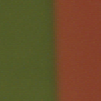
\includegraphics[width=.9\linewidth]{nnCrop2}
  \caption{image 2}
\label{fig:nnCrop2}
\end{subfigure}%
\begin{subfigure}{.25\textwidth}
  \centering
  
\includegraphics[width=.9\linewidth]{nnCrop5}
  \caption{image 5}
\label{fig:nnCrop5}
\end{subfigure}
\caption{A zoomed in area of two NN-interpolation processed images}
\label{fig:nnInterpolation}
\end{figure}


\begin{figure}[H]
\centering
\begin{subfigure}{.25\textwidth}
  \centering
  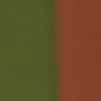
\includegraphics[width=.9\linewidth]{blCrop2}
  \caption{image 2}
\label{fig:blCrop2}
\end{subfigure}%
\begin{subfigure}{.25\textwidth}
  \centering
  
\includegraphics[width=.9\linewidth]{blCrop5}
  \caption{image 5}
\label{fig:blCrop5}
\end{subfigure}
\caption{A zoomed in area of two bilinear interpolation processed images}
\label{fig:blInterpolation}
\end{figure}


\begin{figure}[H]
\centering
\begin{subfigure}{.25\textwidth}
  \centering
  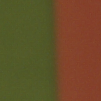
\includegraphics[width=.9\linewidth]{ppgCrop2}
  \caption{image 2}
\label{fig:ppgCrop2}
\end{subfigure}%
\begin{subfigure}{.25\textwidth}
  \centering
  
\includegraphics[width=.9\linewidth]{ppgCrop5}
  \caption{image 5}
\label{fig:ppgCrop5}
\end{subfigure}
\caption{A zoomed in area of two patterned pixel grouping interpolation processed images}
\label{fig:ppgInterpolation}
\end{figure}


The table~\ref{tab:results} contains the Mean Squared Error, Mean Absolute
Error and time it took to run the interpolation function. The error rates were
obtained by processing the raw data with our implemented functions, and
comparing that result to a TIFF encoded file of the same data. The computation
times were obtained using Matlab's tic-toc timetaking function. They'll
depend on the computer used, but what can be objectively compared are their
relative durations.
\begin{table}[H]
  \centering
  \caption{Results from the different methods}
\label{tab:results}
  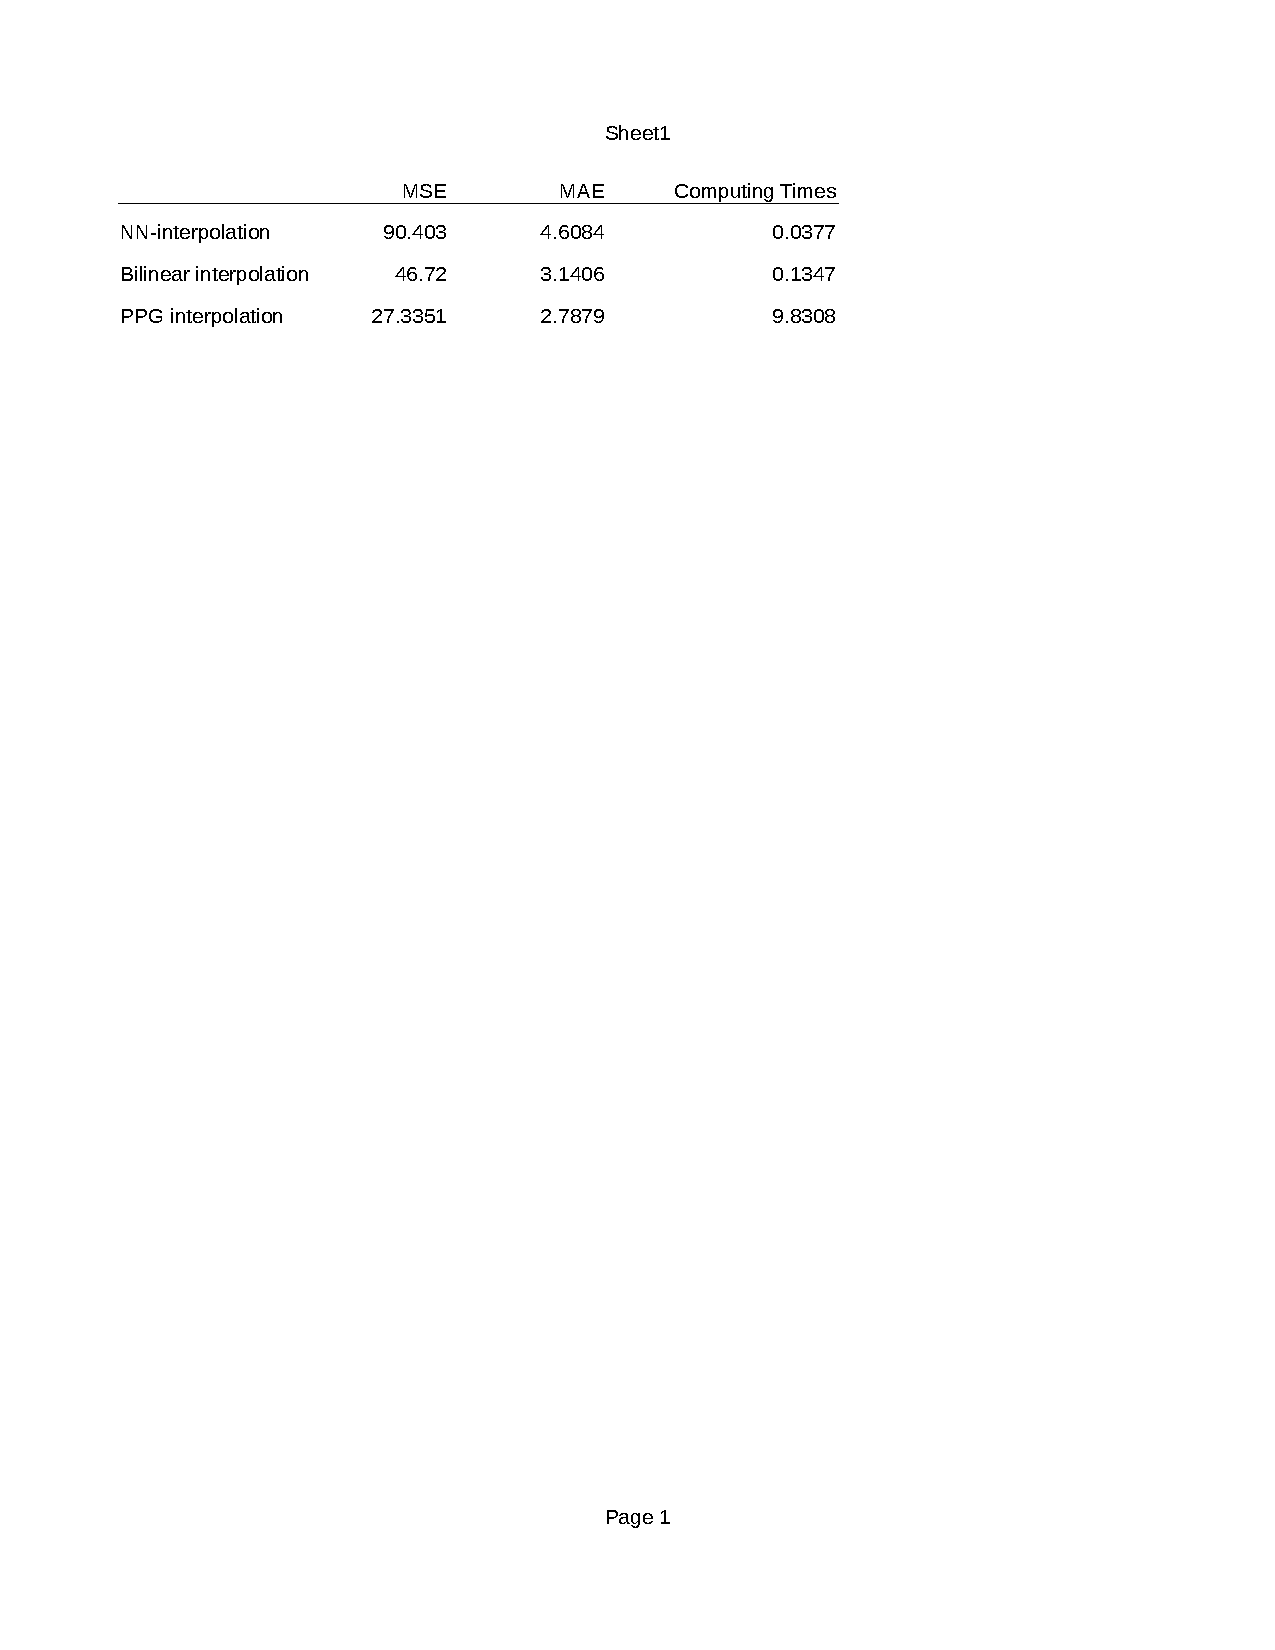
\includegraphics[width=1\linewidth]{results_table}
\end{table}


